\documentclass{beamer}
\usepackage[french]{babel}
\usepackage[T1]{fontenc}
\usepackage[utf8]{inputenc}
\usepackage{media9}

%\usetheme{Madrid}

\title{Introduction à la gestion de version distribuée}
\author{Adrien Plazas\\
	\texttt{kekun.plazas@laposte.net}}
\date{\today}

\begin{document}

\maketitle

\section{Gestion de version}

\begin{frame}{Gestion de version : concepts}
Lorsqu'on travaille sur une projet (seul ou à plusieurs) il est souhaitable de pouvoir :
\begin{itemize}
\item avoir des copies de son travail
\item revenir à des version précédentes
\item faciliter la parallélisation du travail
\end{itemize}

Un gestionnaire de version permet cela.
\end{frame}

\begin{frame}{Gestionnaire de version  en client-serveur}{CVS, Subversion}
\begin{center}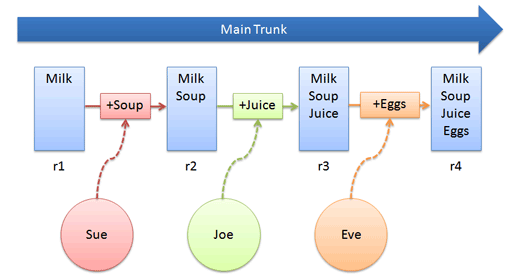
\includegraphics[scale=0.6]{centralized_example.png}\end{center}
\end{frame}

\begin{frame}{Gestionnaire de version distribué}{Bazaar, git, Mercurial}
\begin{center}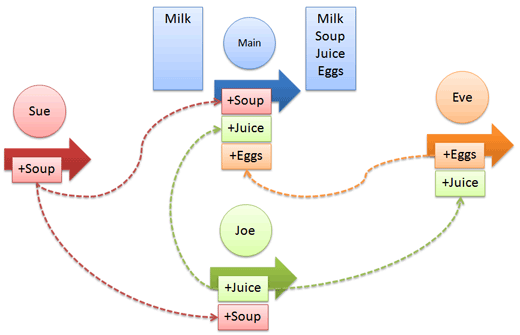
\includegraphics[scale=0.6]{distributed_example.png}\end{center}
\end{frame}

\begin{frame}{Comparaison}
\includemedia{La vidéo ne marche pas}{centralized-vs-distributed.mp4}
\end{frame}

%http://betterexplained.com/articles/intro-to-distributed-version-control-illustrated/


\section{git}

\begin{frame}
\begin{center}
\includegraphics{git-logo.pdf}\end{center}
\end{frame}

\begin{frame}
\begin{quote}git : con, connard, salaud\end{quote}
\begin{flushright}--- WordReference.com\end{flushright}

\begin{quote}Je ne suis qu'un sale égocentrique, donc j'appelle tous mes projets d'après ma propre personne. D'abord Linux, puis Git.\end{quote}
\begin{flushright}--- Linus Torvalds\end{flushright}
\end{frame}

\begin{frame}{Contexte de création}
Linux utilisait BitKeeper

Utilisation de BitKeeper devenue payante $\Rightarrow$ changement de gestionnaire de version
\end{frame}

\begin{frame}{Sélection d'un remplaçant}
Critères requis :
\begin{itemize}
\item fiabilité / robustesse (pas de corruption de dépôt)
\item haute performance (Linux est un gros projet)
\item distribué
\item gratuité
\end{itemize}

Aucun gestionnaire de version viable…
\end{frame}

\begin{frame}{Cahier des charges}
Design : 
\begin{itemize}
	\item Dépôt : graphe orienté acyclique de commissions
	\item Faire l'opposé complet de CVS, s'inspirer de BitKeeper
	\item Suivre non pas des fichiers individuels mais un contenu (tout le dépôt) d'un coup (des fichiers individuels ne sont pas intéressants, une collection de fichiers l'est)
	\item Les commissions sont identifiés par un hash (SHA-1)
	\item Ce hash permet de garantir qu'il n'y a aucune corruption dans le dépôt
\end{itemize}

Création de git par Linus Torvalds (sortie initiale : 7 avril 2005)
\end{frame}

\begin{frame}{Les états}
Les fichiers peuvent être dans trois états pour un dépôt :
\begin{itemize}
	\item Dans le dossier de travail
	\item Dans la zone de préparation
	\item Dans le dépôt
\end{itemize}
\begin{center}
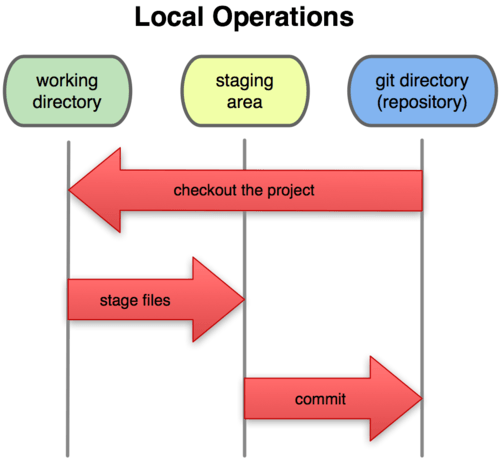
\includegraphics[scale=0.3]{18333fig0106-tn.png}
\end{center}
\end{frame}

\begin{frame}{Cycle de travail classique}{Travail sur une fonctionnalité x}
On crée une branche par fonctionnalité en cours de développement, au nom de la fonctionnalité :
\begin{itemize}
	\item \texttt{git branch x}
\end{itemize}

On se déplace vers cette branche :
\begin{itemize}
	\item \texttt{git checkout x}
\end{itemize}

Lorsqu'on vérifie une branche, le contenu du dossier de travail est remplacé par celui de la branche.

\texttt{master} est la branche par défaut :
\begin{itemize}
	\item \texttt{git checkout master}
\end{itemize}
\end{frame}

\begin{frame}{Cycle de travail classique}{Modification de la branche}
Modifier le dépôt local :

Ajout des nouveaux fichiers et  des fichiers modifiés en zone de préparation :
\begin{itemize}
	\item \texttt{git add fichier1 fichier2}
\end{itemize}

Commission des changements dans le dépôt local (à faire le plus souvent possible) :
\begin{itemize}
	\item \texttt{git commit -m "Message succint décrivant les changements."}
\end{itemize}

Quand la modification est prête :
\begin{itemize}
	\item \texttt{git push}
\end{itemize}

\end{frame}

\begin{frame}{Outils graphiques}
\begin{center}
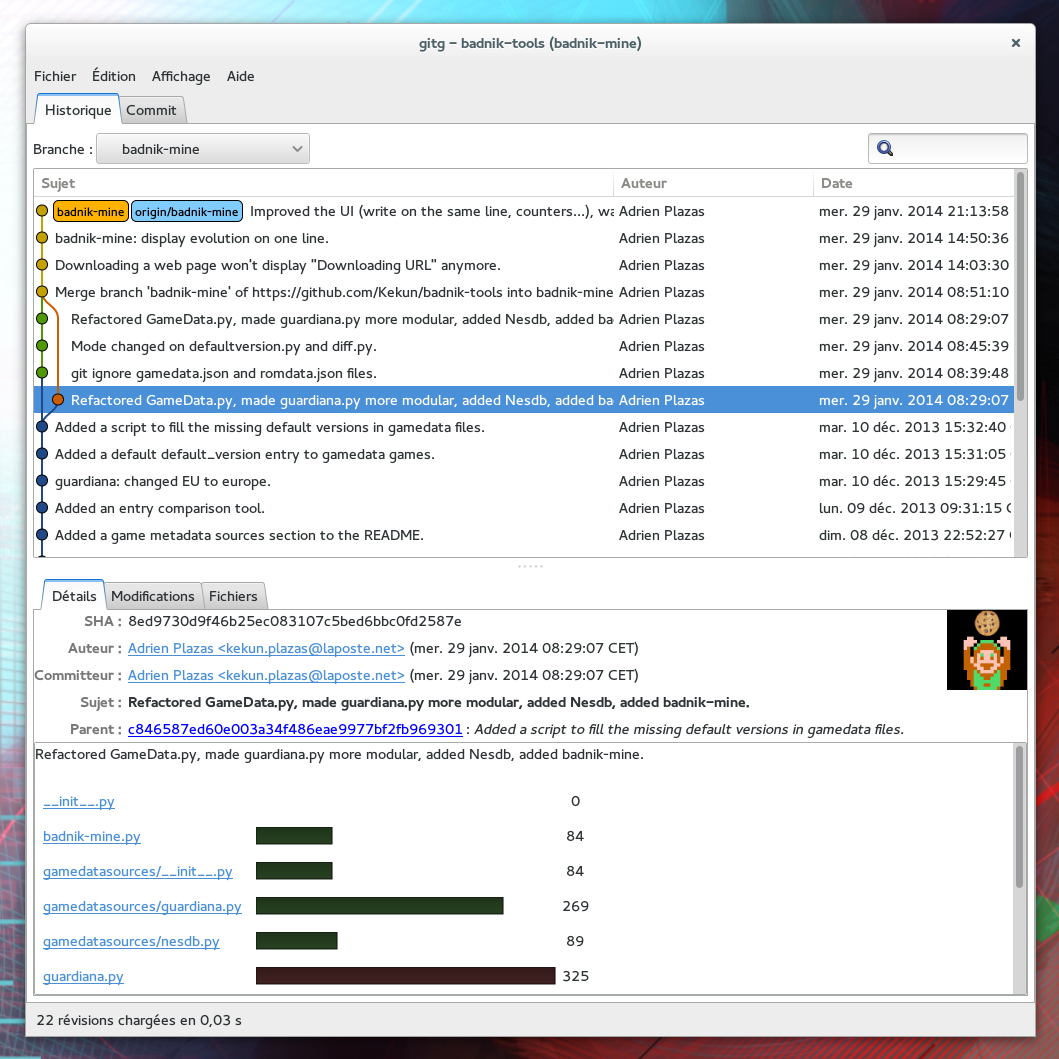
\includegraphics[scale=0.21]{gitg.png}
\end{center}
\end{frame}

\begin{frame}{Essayer git}
http://try.github.io/ permet de tester git en apprenant ses commandes dans un faux terminal.
\end{frame}

%http://try.github.io/


\section{Github}

\begin{frame}
\begin{center}
\includegraphics[scale=0.2]{github-logo.png}
\includegraphics[scale=0.4]{github-logo.pdf}\end{center}
\end{frame}

\begin{frame}
\begin{quote}«~GitHub est un service web d'hébergement et de gestion de développement de logiciels, utilisant le programme Git.~»\end{quote}
\begin{flushright}--- Wikipédia\end{flushright}
\end{frame}

\begin{frame}{Concurrents}

\begin{center}
\includegraphics[scale=0.5]{sourceforge-logo.png}\end{center}

\begin{center}
\includegraphics[scale=0.1]{gitlab-logo.png}{\Huge Gitlab}\end{center}

\end{frame}

\begin{frame}{Gestion de compte}
Il est possible de définir notament :
\begin{itemize}
	\item avatar
	\item pseudo
	\item email
	\item clé SSH (important)
\end{itemize}
\end{frame}

\begin{frame}{Gestion de dépôts}
Github permet de :
\begin{itemize}
	\item Créer des dépôts (https://github.com/new)
	\item Gérer les collaborateurs sur un dépôt
	\item Suivre des dépôts
	\item Fourcher des dépôts
\end{itemize}
\end{frame}

\begin{frame}{Documentation et rapport de bugs}
\begin{itemize}
	\item README.md
	\item Gestionnaire de problèmes
	\item Site web statique (ou Jekyll)
	\item Wiki
\end{itemize}
\end{frame}

\begin{frame}{Autres services}
Gist :
\begin{itemize}
	\item https://gist.github.com/
	\item Partage de petits textes (morceux de code, …)
\end{itemize}

Travis CI :
\begin{itemize}
	\item https://travis-ci.org/
	\item Intégration continue
\end{itemize}
\end{frame}

\begin{frame}{Applications}
Il existes des applications officielles pour :
\begin{itemize}
	\item Windows
	\item Mac OS
	\item Android
\end{itemize}
\begin{center}
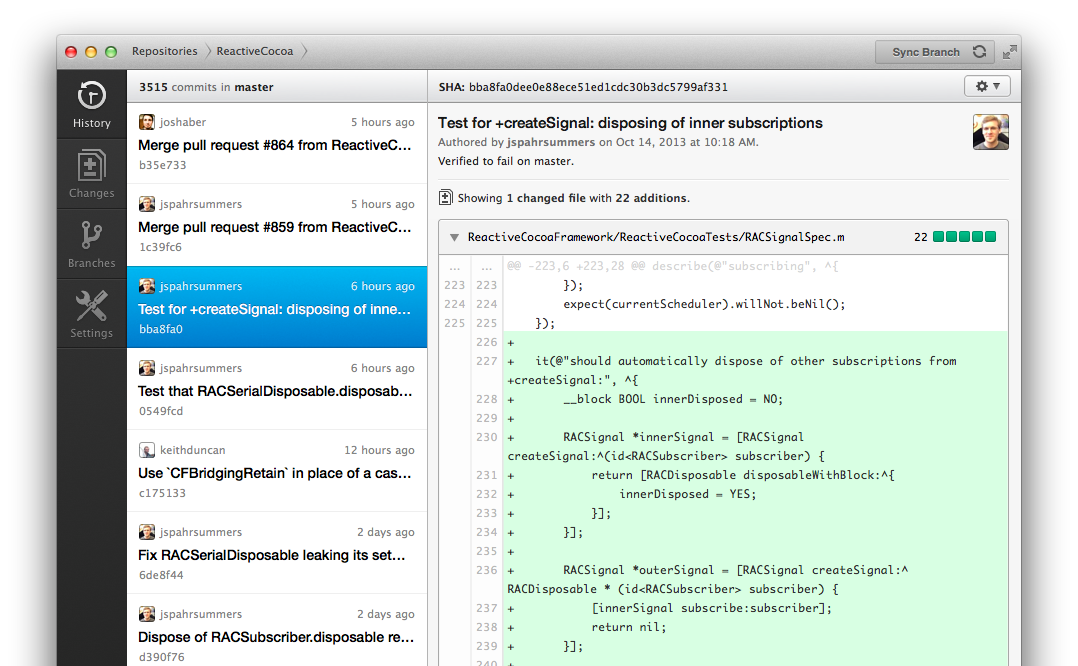
\includegraphics[scale=0.3]{screen1.png}
\end{center}
\end{frame}



% sources
% http://www.youtube.com/watch?v=4XpnKHJAok8
% http://en.wikipedia.org/wiki/Git
% http://en.wikipedia.org/wiki/Github
% http://betterexplained.com/articles/intro-to-distributed-version-control-illustrated/
% http://www.youtube.com/watch?v=_yQlKEq-Ueg

\end{document}

